	% Vita of Author
% Argument 1: info about the author
% Argument 2: author photograph 
% Argument 3: Contact information of the author

\vita{
%This is where you put information about the author
%Saroj Snehal Shivagunde obtained her degree of B.E. from Saraswati College of Engineering, Navi Mumbai and her M.Tech. degree from Indian Institute of Technology, Guwahati (IITG). She is currently a Ph.D. student at IITG under the supervision of Dr. Vijaya Saradhi Vedula. Her research interests include multi-view and incremental learning.
%\input{./Vitae_Full/CV.pdf}
%\begin{figure*}[t]
%	\centering
%	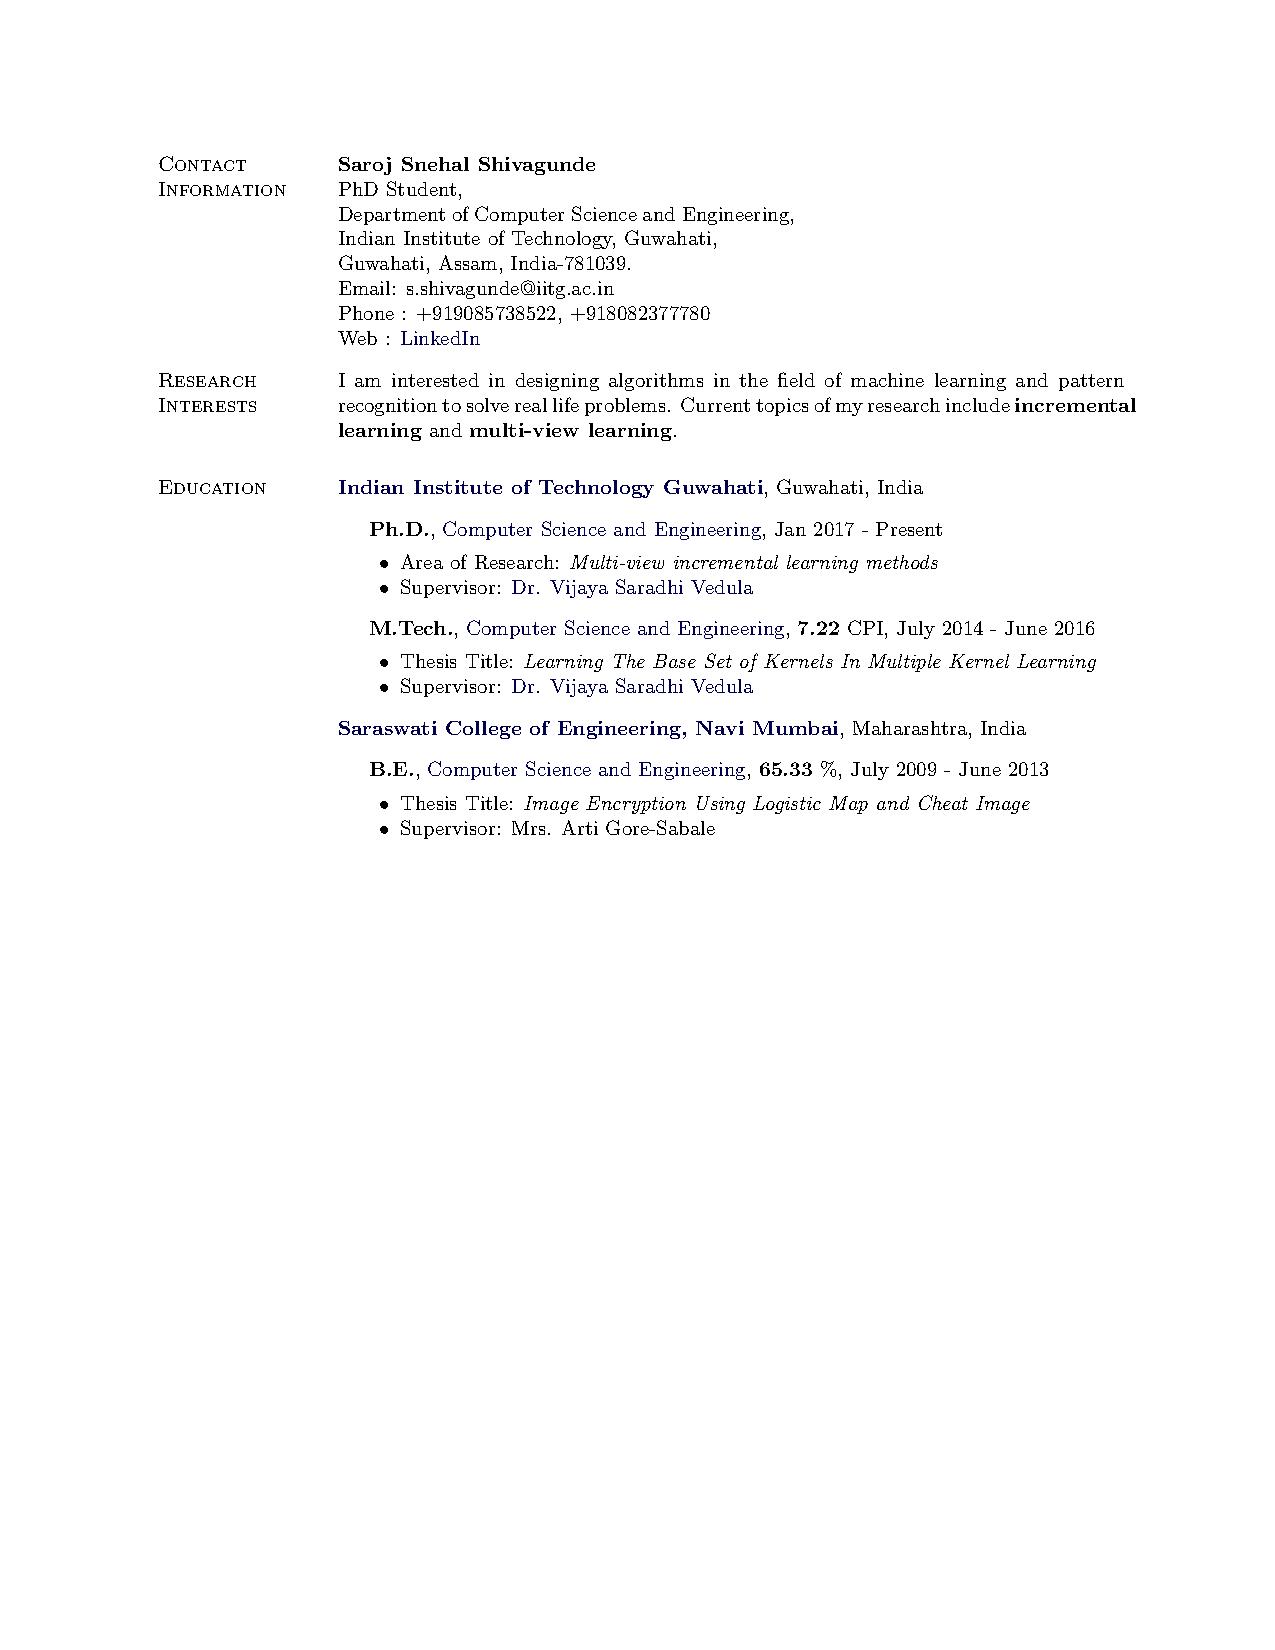
\includegraphics[width=\textwidth]{CV.pdf}
%\end{figure*}


\begin{tabular}{p{0.8in}p{5in}}
\multicolumn{2}{l}{\textbf{Saroj Snehal Shivagunde}} \\
%\textbf{Name} & Saroj Snehal Shivagunde \\
& \\
{\small\textbf{Current}} & PhD Student, Department of Computer Science and Engineering,\\ 
{\small\textbf{Affiliation}} & Indian Institute of Technology, Guwahati, India. \\
& \\
\textbf{Email} 	& s.shivagunde@iitg.ac.in,\\ 
				& sarojshivagunde@gmail.com \\
& \\
\textbf{Web} & \href{https://www.linkedin.com/in/saroj-shivagunde}{LinkedIn}, \href{https://github.com/SarojShivagunde/MvIDA}{GitHub}\\
& \\
\textbf{Research}  & I am interested in designing algorithms in the field of machine learning and\\
\textbf{Interests} & pattern recognition to solve real life problems. Current topics of my research\\
				   & include \textbf{incremental learning} and \textbf{multi-view learning}.\\
& \\
\textbf{Education}  & \textbf{M.Tech, Computer Science and Engineering, 2014-2016}\\
					& Indian Institute of Technology, Guwahati\\
					& Thesis Title : \emph{Learning The Base Set of Kernels In Multiple Kernel Learning}\\
					& Supervisor : Dr. Vijaya Saradhi Vedula\\
& \\
					& \textbf{B.E., Computer Science and Engineering, 2009-2013}\\
					& Saraswati College of Engineering, Navi Mumbai\\
					& Thesis Title : \emph{Image Encryption Using Logistic Map and Cheat Image}\\
					& Supervisor : Mrs. Arti Gore-Sabale\\
& \\
\end{tabular}


\chapterend
}
%{% place the path of your photograph here within braces without any extra space or return -> {Path_to_Figure}
%\begin{minipage}[t]{0.95\textwidth}
%	\begin{figure}[t]
%		\centering
%		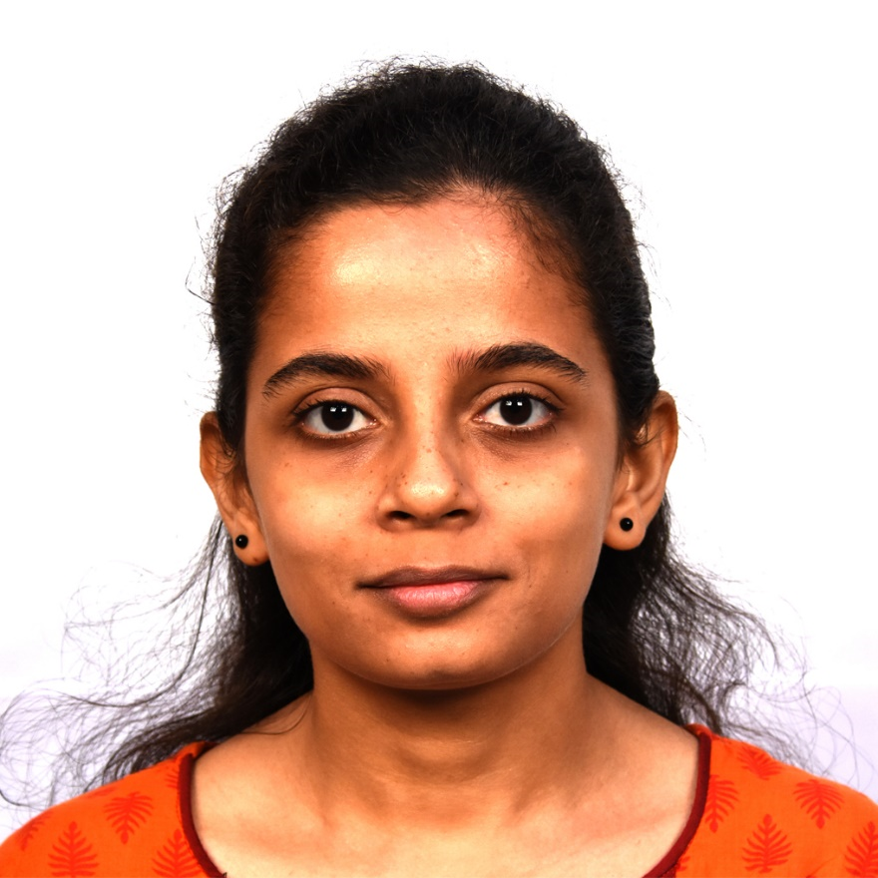
\includegraphics[width=0.4\textwidth]{Figures/Photograph.png}
%	\end{figure}
%\end{minipage}
% This argument is for the contact address of the author (you can provide address, email id, etc. in this section)

%\begin{tabular}{p{2in}p{0.5in}p{4in}}
%\textbf{Email} & : & s.shivagunde@iitg.ac.in,\\ 
%& & sarojshivagunde@gmail.com \\
%%& & \\
%\textbf{Web} & : & \href{https://www.linkedin.com/in/saroj-shivagunde}{LinkedIn}\\
%& & \\
%\textbf{Address} &:& \\
%& & \\
%\end{tabular}

%}